\newpage
\section{CƠ SỞ DỮ LIỆU}
\subsection{Mô hình thực thể liên kết mở rộng (EERD)}
\begin{figure}[H]
    \centering
    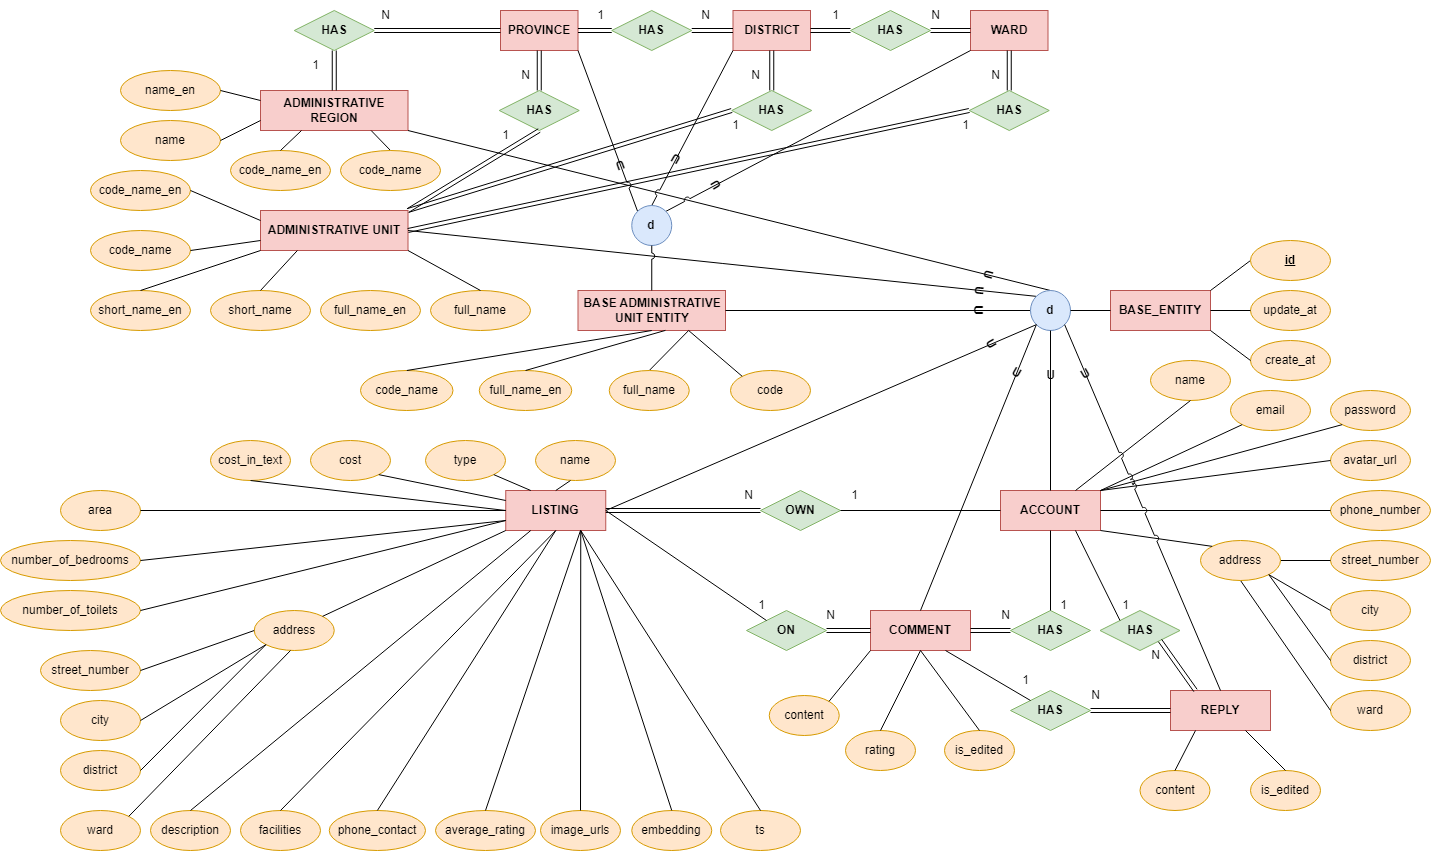
\includegraphics[angle=270,width=0.7\textwidth]{Images/Database/ERD.png}
    \caption{Thiết kế ERD cho cơ sở dữ liệu}
\end{figure}
\subsection{Mô tả thiết kế}
\subsubsection{Các kiểu thực thể}
Trong mô hình EERD trên có 10 thực thể được mô tả như sau:
\begin{itemize}
    \item \textbf{BASE\_ENTITY}: Đây là kiểu thực thể tổng quát để lưu trữ các thuộc tính cần phải được lưu trữ trong các kiểu thực thể còn lại. Các thuộc tính được lưu trữ của kiểu thực thể này bao gồm:
    \begin{itemize}
        \item \underline{\textit{\bf id}}: Thuộc tính khóa dùng để phân biệt các thực thể với nhau trong một kiểu thực thể nhất định.
        \item \textit{create\_at}: Thuộc tính để lưu trữ thời điểm ban đầu mà thực thể dược khởi tạo.
        \item \textit{updated\_at}: Thuộc tính dùng để ghi nhận thời điểm mà thực thể có sự thay đổi ở các thuộc tính.
    \end{itemize}
    \item \textbf{BASE\_ADMINISTRATIVE\_UNIT\_ENTITY}: Đây là kiểu thực thể dùng để lưu trữ các thuộc tính sử dụng chung cho các thực thể \textit{PROVINCE}, \textit{DISTRICT} VÀ \textit{WARD}. Thực thể này có sự kế thừa các thuộc tính từ thực thể \textit{BASE\_ENTITY}. Các thuộc tính được lưu trữ của kiểu thực thể này bao gồm:
    \begin{itemize}
        \item \textit{code}: Mỗi một đơn vị hành chính sẽ có một mã định dang duy nhất được quy định bởi chính phủ Việt Nam
        \item \textit{full\_name}: Tên đầy đủ của đơn vị hành chính bằng tiếng Việt
        \item \textit{full\_name\_en}: Tên đầy đủ của đơn vị hành chính bằng tiếng Anh
        \item \textit{code\_name}: Tên chuẩn hóa của đơn vị hành chính
    \end{itemize}
    \item \textbf{ADMINISTRATIVE\_UNIT}: Đây là kiểu thực thể dùng để lưu trữ các loại cấp bậc của phân cấp đơn vị hành chính trên lãnh thổ Việt Nam. Thực thể này có sự kế thừa các thuộc tính từ thực thể \textit{BASE\_ENTITY}. Các thuộc tính được lưu trữ của kiểu thực thể này bao gồm:
    \begin{itemize}
        \item \textit{full\_name}: Tên đầy đủ của loại cấp bậc đơn vị hành chính bằng tiếng Việt
        \item \textit{full\_name\_en}: Tên đầy đủ của loại cấp bậc của đơn vị hành chính bằng tiếng Anh
        \item \textit{short\_name}: Tên ngắn gọn của loại cấp bậc đơn vị hành chính bằng tiếng Việt
        \item \textit{short\_name\_en}: Tên ngắn của loại cấp bậc của đơn vị hành chính bằng tiếng Anh
        \item \textit{code\_name}: Tên chuẩn hóa của loại cấp bậc đơn vị hành chính bằng tiếng Việt
        \item \textit{code\_name\_en}: Tên chuẩn hóa của loại cấp bậc đơn vị hành chính bằng tiếng Anh
    \end{itemize}
    \item \textbf{ADMINISTRATIVE\_REGION}: Đây là kiểu thực thể dùng để lưu trữ các vùng kinh tế - xã hội trên lãnh thổ Việt Nam. Thực thể này có sự kế thừa các thuộc tính từ thực thể \textit{BASE\_ENTITY}. Các thuộc tính được lưu trữ của kiểu thực thể này bao gồm:
    \begin{itemize}
        \item \textit{name}: Tên đầy đủ của vùng kinh tế - xã hội bằng tiếng Việt
        \item \textit{name\_en}: Tên đầy đủ của vùng kinh tế - xã hội bằng tiếng Anh
        \item \textit{code\_name}: Tên chuẩn hóa của vùng kinh tế - xã hội bằng tiếng Việt
        \item \textit{code\_name\_en}: Tên chuẩn hóa của vùng kinh tế - xã hội bằng tiếng Anh
    \end{itemize}
    \item \textbf{PROVINCE}: Đây là kiểu thực thể dùng để lưu trữ toàn bộ các tỉnh / thành phố trên lãnh thổ Việt Nam. Thực thể này có sự kế thừa các thuộc tính từ các thực thể \textit{BASE\_ENTITY} và \textit{BASE\_ADMINISTRATIVE\_UNIT\_ENTITY}.
    \item \textbf{DISTRICT}: Đây là kiểu thực thể dùng để lưu trữ toàn bộ các quận / huyện và các đơn vị hành chính cấp tương đương trên lãnh thổ Việt Nam. Thực thể này có sự kế thừa các thuộc tính từ các thực thể \textit{BASE\_ENTITY} và \textit{BASE\_ADMINISTRATIVE\_UNIT\_ENTITY}.
    \item \textbf{ward}: Đây là kiểu thực thể dùng để lưu trữ toàn bộ các phường / xã và các đơn vị hành chính cấp tương đương trên lãnh thổ Việt Nam. Thực thể này có sự kế thừa các thuộc tính từ các thực thể \textit{BASE\_ENTITY} và \textit{BASE\_ADMINISTRATIVE\_UNIT\_ENTITY}.
    \item \textbf{ACCOUNT}: Đây là kiểu thực thể dùng để lưu thông tin người dùng sử dụng ứng dụng, người dùng này có thể là người chủ trọ đăng bài thuê trọ và cũng có thể là người có nhu cầu sử dụng ứng dụng để thuê trọ. Thực thể này có sự kế thừa các thuộc tính từ thực thể \textit{BASE\_ENTITY}. Các thuộc tính được lưu trữ của kiểu thực thể này bao gồm:
    \begin{itemize}
        \item \textit{name}: Là tên của người dùng, bao gồm cả họ và tên.
        \item \textit{email}: Là địa chỉ email mà người dùng sử dụng để đăng ký tài khoản cho ứng dụng.
        \item \textit{password}: Là mật khẩu mà người dùng khởi tạo khi đăng ký tài khoản ứng dụng. Trong cơ sở dữ liệu, mật khẩu của người dùng sẽ được băm một chiều nên chỉ có người dùng mới có thể biết được thông tin của mật khẩu.
        \item \textit{phone\_number}: Là số điện thoại mà người dùng có thể ghi nhận đăng ký khi khởi tạo tài khoản, số điện thoại này có thể được dùng để công khai khi người dùng đăng bài viết cho thuê nhà trọ.
        \item \textit{avatar\_url}: Là đường dẫn ứng với hình ảnh đại diện của người dùng, file hình ảnh sẽ được lưu trữ trên dịch vụ lưu trữ đám mây, dịch vụ này sẽ trả về đường dẫn ứng với file hình ảnh đó để lưu trữ trong cơ sở dữ liệu.
        \item \textit{address}: Là địa chỉ sinh sống của người dùng ở thời điểm hiện tại, người dùng có thể tùy ý cung cấp thông tin về địa chỉ cho ứng dụng hoặc không. Thuộc tính \textit{address} bao gồm sự kết hợp của 4 thuộc tính theo phân cấp đơn vị hành chính của Việt Nam như sau:
        \begin{itemize}
            \item \textit{city}: Là tỉnh / thành phố của địa chỉ người dùng
            \item \textit{district}: Là quận / huyện hoặc đơn vị hành chính cấp tương đương của địa chỉ người dùng
            \item \textit{ward}: Là phường / xã hoặc đơn vị hành chính cấp tương đương của địa chỉ người dùng
            \item \textit{street\_number}: Bao gồm số nhà và tên đường / hẻm của địa chỉ người dùng
        \end{itemize}
    \end{itemize}
    \item \textbf{LISTING}: Là kiểu thực thể để lưu trữ thông tin bài đăng tải nhà thuê, thực thể này bao gồm các thuộc tính lưu trữ những thông tin liên quan đến một nhà trọ mà người sử dụng ứng dụng quan tâm khi tìm kiếm, đồng thời cũng lưu trữ các thuộc tính riêng để thực hiện triển khai tìm kiếm trên mô hình Hybrid. Thực thể này có sự kế thừa các thuộc tính từ thực thể \textit{BASE\_ENTITY}. Các thuộc tính được lưu trữ của kiểu thực thể này bao gồm:
    \begin{itemize}
        \item \textit{name}: Tiêu đề của của bài đăng tải nhà thuê.
        \item \textit{type}: Là loại hình cho thuê nhà, cơ sở dữ liệu cho phép người đăng tải được chọn một trong ba loại hình cho thuê bao gồm: \textit{Phòng trọ}, \textit{Căn hộ} hoặc \textit{Nhà đất}.
        \item \textit{cost}: Giá cho thuê nhà theo tháng
        \item \textit{cost\_in\_text}: Giá cho thuê nhà theo tháng được phiên âm thành tiếng Việt. Thuộc tính này nhằm mục đích biểu thị ngữ nghĩa của giá cho thuê nhà trọ để có thể sử dụng tốt trong mô hình tìm kiếm Hybrid.
        \item \textit{area}: Thông tin về diện tích của nhà thuê.
        \item \textit{number\_of\_bedrooms}: Số lượng phòng ngủ.
        \item \textit{number\_of\_toilets}: Số lượng nhà vệ sinh.
        \item \textit{cost}: Giá cho thuê theo tháng.
        \item \textit{cost\_in\_text}: Giá cho thuê theo tháng được phiên âm thành tiếng Việt. Thuộc tính này được lưu trữ nhằm mục đích chuyển đổi từ số sang ngữ nghĩa để sử dụng trong mô hình tìm kiếm hybrid.
        \item \textit{address}: Là địa chỉ của nhà trọ. Tương tự như kiểu thực thể \textbf{ACCOUNT}, thuộc tính \textit{address} bao gồm sự kết hợp của 4 thuộc tính theo phân cấp đơn vị hành chính của Việt Nam như sau:
        \begin{itemize}
            \item \textit{city}: Là tỉnh / thành phố của địa chỉ nhà thuê.
            \item \textit{district}: Là quận / huyện hoặc đơn vị hành chính cấp tương đương của nhà thuê
            \item \textit{ward}: Là phường / xã hoặc đơn vị hành chính cấp tương đương của nhà thuê
            \item \textit{street\_number}: Bao gồm số nhà và tên đường / hẻm ứng với địa chỉ của nhà thuê
        \end{itemize}
        \item \textit{description}: Mô tả ngắn về bài đăng cho thuê nhà.
        \item \textit{facilities}: Các tiện ích của nhà trọ cho thuê, bao gồm danh sách các tiện ích đã được quy ước sẵn trong ứng dụng như: \textit{Tivi}, \textit{Camera giám sát}, \textit{Cảm biến thông minh}, \textit{Máy giặt}, \textit{Tủ lạnh}, \textit{Điều hòa}.
        \item \textit{phone\_contact}: Số điện thoại liên hệ để người sử dụng có thể tiếp cận được với chủ bài đăng.
        \item \textit{average\_rating}: Điểm trung bình của nhà thuê được tính toán dựa trên tất cả các bình luận và đánh giá do những người khác cung cấp cho bài đăng.
        \item \textit{image\_urls}: Lưu trữ các đường dẫn của hình ảnh về nhà thuê để hiển thị khi người dùng xem chi tiết về thông tin bài đăng tải.
        \item \textit{ts}: Thuộc tính dùng để lưu trữ các chỉ mục \textit{indexes} của tất cả các từ ngữ trong bài đăng tải nhà thuê. Thuộc tính này lưu trữ nhằm dùng để phục vụ cho \textit{full-text search}.
        \item \textit{embedding}: Thuộc tính dùng để lưu trữ thông tin ngữ nghĩa về bài đăng nhà thuê dưới dạng \textit{vector}, được sinh ra bởi mô hình \textit{vector embedding}, Thuộc tính này lưu trữ nhằm dùng để phục vụ cho \textit{semantic search}
    \end{itemize}
    \item \textbf{COMMENT}: Kiểu thực thể lưu trữ các bình luận của người dùng đối với một bài đăng tải nhà thuê nhất định. Thực thể này có sự kế thừa các thuộc tính từ thực thể \textit{BASE\_ENTITY}. Các thuộc tính được lưu trữ của kiểu thực thể này bao gồm:
    \begin{itemize}
        \item \textit{content}: Nội dung của bình luận.
        \item \textit{rating}: Điểm đánh giá của người dùng từ 1 đến 5 sao.
        \item \textit{is\_edited}: Biểu thị cho việc người dùng đã chỉnh sửa bình luận hay không.
    \end{itemize}
    \item \textbf{REPLY}: Kiểu thực thể lưu trữ các phản hồi của người dùng cho một bình luận nhất định. Thực thể này có sự kế thừa các thuộc tính từ thực thể \textit{BASE\_ENTITY}. Các thuộc tính được lưu trữ của kiểu thực thể này bao gồm:
    \begin{itemize}
        \item \textit{content}: Nội dung của phản hồi bình luận.
        \item \textit{is\_edited}: Biểu thị cho việc người dùng đã chỉnh sửa phản hồi hay không.
    \end{itemize}
\end{itemize}
\subsubsection{Các mối liên kết}
Các thực thể trong mô hình EERD tồn tại các mối liên kết sau:
\begin{itemize}
    \item ADMINISTRATIVE\_UNIT \textbf{HAS} PROVINCE: Đây là mối liên kết \textit{one - to - many} để biểu thị cho việc một đơn vị hành chính (ở đây là tỉnh, thành phố) phải liên kết với tất cả các tỉnh / thành phố trực thuộc trung ương trên lãnh thổ Việt Nam. Mối liên kết trên có ý nghĩa là tỉnh / thành phố trực thuộc trung ương trong đơn vị phân cấp hành chính phải có sự liên kết đối với tất cả các tỉnh / thành phố trực thuộc trung ương của Việt Nam, và ngược lại, tất cả các tỉnh / thành phố trực thuộc trung ương đều phải được phân loại vào đơn vị hành chính là tỉnh / thành phố trực thuộc trung ương.
    \item ADMINISTRATIVE\_UNIT \textbf{HAS} DISTRICT: Đây là mối liên kết \textit{one - to - many} để biểu thị cho việc một đơn vị hành chính (ở đây là quận / huyện hoặc đơn vị hành chính cấp tương đương) phải liên kết với tất cả các quận / huyện hoặc đơn vị hành chính cấp tương đương trên lãnh thổ Việt Nam. Mối liên kết trên có ý nghĩa là quận / huyện hoặc đơn vị hành chính cấp tương đương trong đơn vị phân cấp hành chính phải có sự liên kết đối với tất cả các quận / huyện hoặc đơn vị hành chính cấp tương đương của Việt Nam, và ngược lại, tất cả các quận / huyện hoặc đơn vị hành chính cấp tương đương đều phải được phân loại vào đơn vị hành chính là quận / huyện hoặc đơn vị hành chính cấp tương đương.
    \item ADMINISTRATIVE\_UNIT \textbf{HAS} WARD: Đây là mối liên kết \textit{one - to - many} để biểu thị cho việc một đơn vị hành chính (ở đây là phường / xã hoặc đơn vị hành chính cấp tương đương) phải liên kết với tất cả các phường / xã hoặc đơn vị hành chính cấp tương đương trên lãnh thổ Việt Nam. Mối liên kết trên có ý nghĩa là phường / xã hoặc đơn vị hành chính cấp tương đương trong đơn vị phân cấp hành chính phải có sự liên kết đối với tất cả các phường / xã hoặc đơn vị hành chính cấp tương đương của Việt Nam, và ngược lại, tất cả các phường / xã hoặc đơn vị hành chính cấp tương đương đều phải được phân loại vào đơn vị hành chính là phường / xã hoặc đơn vị hành chính cấp tương đương.
    \item ADMINISTRATIVE\_REGION \textbf{HAS} PROVINCE: Đây là mối liên kết \textit{one - to - many} để biểu thị cho việc một vùng kinh tế - xã hội phải liên kết với tất cả các tỉnh / thành phố trên phạm vi của vùng kinh tế - xã hội đó. Mối liên kết trên có ý nghĩa là mỗi vùng kinh tế - xã hội phải có nhiều tỉnh / thành phố trực thuộc trung ương, và ngược lại, tất cả các tỉnh / thành phố trực thuộc trung ương trên lãnh thổ Việt Nam đều phải được thuộc về một vùng kinh tế - xã hội nhất định.
    \item PROVINCE \textbf{HAS} DISTRICT: Đây là mối liên kết \textit{one - to - many} để biểu thị cho việc một tỉnh / thành phố trực thuộc trung ương phải liên kết với nhiều quận / huyện hoặc đơn vị hành chính cấp tương đương trên phạm vi của tỉnh / thành phố đó. Mối liên kết trên có ý nghĩa là tỉnh / thành phố phải có nhiều quận / huyện hoặc đơn vị hành chính cấp tương đương, và ngược lại, tất cả các quận / huyện hoặc đơn vị hành chính cấp tương đương đều phải thuộc về một tỉnh / thành phố nhất định.
    \item DISTRICT \textbf{HAS} WARD: Đây là mối liên kết \textit{one - to - many} để biểu thị cho việc một quận / huyện hoặc đơn vị hành chính cấp tương đương phải liên kết với nhiều phường / xã hoặc đơn vị hành chính cấp tương đương trên phạm vi của quận / huyện đó. Mối liên kết trên có ý nghĩa là quận / huyện hoặc đơn vị hành chính cấp tương đương phải có nhiều phường / xã hoặc đơn vị hành chính cấp tương đương, và ngược lại, tất cả các phường / xã hoặc đơn vị hành chính cấp tương đương đều phải thuộc về một quận / huyện hoặc đơn vị hành chính cấp tương đương nhất định.
    \item ACCOUNT \textbf{OWN} LISTING: Đây là mối liên kết \textit{one - to - many} để biểu thị cho việc một tài khoản người dùng được liên kết tới nhiều bài đăng nhà thuê cho ứng dụng. Ở đây, mối liên kết này có ý nghĩa là một tài khoản người dùng không nhất thiết phải có bài đăng tải nhà thuê, tuy nhiên ngược lại tất cả các bài đăng nhà thuê đều phải thuộc về một người dùng nhất định.
    \item COMMENT \textbf{ON} LISTING: Đây là mối liên kết \textit{many - to - one} để biểu thị cho việc các bình luận sẽ được liên kết với các bài đăng tải nhà thuê. Mối liên kết này có ý nghĩa là một bài đăng tải nhà thuê có thể không có hoặc có nhiều bình luận, tuy nhiên ngược lại thì bất kì một bình luận nào cũng phải thuộc về một bài đăng nhất định.
    \item ACCOUNT \textbf{HAS} COMMENT: Đây là mối liên kết \textit{one - to - many} để biểu thị cho việc một người dùng sẽ được liên kết tới tất cả các bình luận mà người dùng đó để lại trên các bài đăng tải nhà thuê nhất định. Ở đây mối liên kết này có ý nghĩa là một người dùng có thể không có hoặc có nhiều bình luận, và các bình luận này có thể thuộc về một hoặc nhiều bài đăng tải nhà trọ nhất định, tuy nhiên ngược lại, bất kì một bình luận nào cũng đều phải thuộc về một người dùng nhất định.
    \item COMMENT \textbf{HAS} REPLY: Đây là mối liên kết \textit{one - to - many} để biểu thị cho việc một bình luận được liên kết tới nhiều phần phản hồi cho bình luận đó. Ở đây mối liên kết này có ý nghĩa là một bình luận nhất định có thể không có hoặc có nhiều phần phản hồi ở phía dưới, tuy nhiên ngược lại, bất kì một phản hồi bình luận nào cũng đều phải thuộc về một bình luận nhất định.
    \item ACCOUNT \textbf{HAS} REPLY: Đây là mối liên kết \textit{one - to - many} để biểu thị cho việc một người dùng sẽ được liên kết tới tất cả các phản hồi bình luận mà người dùng đó để lại trên các bình luận nhất định. Ở đây mối liên kết này có ý nghĩa là một người dùng có thể không có hoặc có nhiều phản hồi cho các bình luận, và các phản hồi này có thể thuộc về một hoặc nhiều bình luận nhất định, tuy nhiên ngược lại, bất kì một phần phản hồi bình luận nào cũng đều phải thuộc về một người dùng nhất định.
\end{itemize}
\subsection{Ánh xạ qua cơ sở dữ liệu PostgreSQL bằng Prisma ORM}
\subsubsection{Tổng quan}
\hspace*{1cm}
Để đơn giản hóa quy trình làm việc với cơ sở dữ liệu, các thư viện hay \textit{framework} để xây dựng \textit{Web API} thường sẽ cung cấp một lớp trung gian để làm việc với cơ sở dữ liệu ở bên dưới được gọi là \textit{Object Relational Mapping} hay còn được gọi gọi đơn giản là \textit{ORM}. Điều này sẽ giúp cho các nhà phát triển có thể thao tác, thực hiện các truy vấn cơ sở dữ liệu bằng chính ngôn ngữ lập trình mà không cần phải sử dụng \textit{SQL} theo cách truyền thống. Có nhiều lợi ích có thể thấy được với \textit{ORM} mà có hai điều dễ nhận thấy nhất, đầu tiên là các nhà phát triển không cần phải quan tâm quá nhiều tới hiện thực của cơ sở dữ liệu ở bên dưới, mà chỉ cần thông qua các \textit{API} do \textit{ORM} cung cấp, giúp cho các nhà phát triển tập trung nhiều hơn cho việc phát triển các chức năng chính của ứng dụng và tối thiểu hóa những sai sót liên quan đến việc thao tác với cơ sở dữ liệu, tuy nhiên do các hệ quản trị cơ sở dữ liệu có những khác biệt đặc thù với nhau, nên trong một vài tình huống nhất định, nhà phát triển cũng cần phải quan tâm tới hệ quản trị cơ sở dữ liệu một cách cụ thể. Lợi ích thứ hai rất dễ để nhận thấy đó là khi làm việc thông qua \textit{ORM}, các nhà phát triển có thể tối thiểu hóa các lỗ hổng bảo mật liên quan tới cơ sở dữ liệu, và một trong các lỗ hổng phổ biến nhất đó là \textit{SQL Injections}, khi kẻ xấu phát hiện ra được lỗ hổng này và khai thác được thì hậu quả gây ra cho cơ sở dữ liệu có thể rất nghiêm trọng.\\
\hspace*{1cm}
Để chuyển đổi mô hình thực thể liên kết đã được trình bày phía trên thành hiện thực cơ sở dữ liệu ở bên dưới ứng dụng. Nhóm sử dụng \textit{Prisma ORM}, đây có thể được coi là thư viện \textit{ORM} dành cho các ứng dụng \textit{Node.js} và có thể hỗ trợ các hệ quản trị cơ sở dữ liệu phổ biến nhất hiện nay, bao gồm cả \textit{SQL} và \textit{NoSQL}. Chi tiết về \textit{Prisma} sẽ được trình bày chi tiết hơn trong phần phía dưới. Ở đây, để đặc tả cơ sở dữ liệu dựa trên mô hình thực thể liên kết, nhóm sẽ tạo một \textit{file} tên là \textit{schema.prisma} trong mã nguồn ở phía \textit{back-end}, file này sẽ được dùng để mô tả các bảng và quan hệ và sau đó sẽ được ánh xạ sang cơ sở dữ liệu ở bên dưới.
\subsubsection{Ánh xạ chi tiết các bảng}
{\scriptsize
\begin{lstlisting}[caption={Ánh xạ bảng AdministrativeRegion},captionpos=b]
model AdministrativeRegion {
  id         Int        @id @default(autoincrement())
  createAt   DateTime   @default(now()) @map("create_at")
  updatedAt  DateTime   @default(now()) @updatedAt @map("updated_at")
  name       String     @db.VarChar(255)
  nameEn     String     @map("name_en") @db.VarChar(255)
  codeName   String?    @map("code_name") @db.VarChar(255)
  codeNameEn String?    @map("code_name_en") @db.VarChar(255)
  Provinces  Province[]

  @@map("administrative_regions")
}
\end{lstlisting}}
{\scriptsize
\begin{lstlisting}[caption={Ánh xạ bảng AdministrativeUnit},captionpos=b]
model AdministrativeUnit {
  id          Int        @id @default(autoincrement())
  createAt    DateTime   @default(now()) @map("create_at")
  updatedAt   DateTime   @default(now()) @updatedAt @map("updated_at")
  fullName    String?    @map("full_name") @db.VarChar(255)
  fullNameEn  String?    @map("full_name_en") @db.VarChar(255)
  shortName   String?    @map("short_name") @db.VarChar(255)
  shortNameEn String?    @map("short_name_en") @db.VarChar(255)
  codeName    String?    @map("code_name") @db.VarChar(255)
  codeNameEn  String?    @map("code_name_en") @db.VarChar(255)
  Provinces   Province[]
  Districts   District[]
  Wards       Ward[]

  @@map("administrative_units")
}
\end{lstlisting}}
{\scriptsize
\begin{lstlisting}[caption={Ánh xạ bảng Province},captionpos=b]
model Province {
  id                     Int                   @id @default(autoincrement())
  createAt               DateTime              @default(now()) @map("create_at")
  updatedAt              DateTime              @default(now()) @updatedAt @map("updated_at")
  code                   String                @unique @db.VarChar(20)
  name                   String                @db.VarChar(255)
  nameEn                 String?               @map("name_en") @db.VarChar(255)
  fullName               String                @map("full_name") @db.VarChar(255)
  fullNameEn             String?               @map("full_name_en") @db.VarChar(255)
  codeName               String?               @map("code_name") @db.VarChar(255)
  codeNameEn             String?               @map("code_name_en") @db.VarChar(255)
  administrativeUnitId   Int?                  @map("administrative_unit_id")
  administrativeRegionId Int?                  @map("administrative_region_id")
  AdministrativeUnit     AdministrativeUnit?   @relation(fields: [administrativeUnitId], references: [id])
  AdministrativeRegion   AdministrativeRegion? @relation(fields: [administrativeRegionId], references: [id])
  Districts              District[]

  @@index([administrativeRegionId, administrativeUnitId])
  @@map("provinces")
}
\end{lstlisting}}
{\scriptsize
\begin{lstlisting}[caption={Ánh xạ bảng District},captionpos=b]
model District {
  id                   Int                 @id @default(autoincrement())
  createAt             DateTime            @default(now()) @map("create_at")
  updatedAt            DateTime            @default(now()) @updatedAt @map("updated_at")
  code                 String              @unique @db.VarChar(20)
  name                 String              @db.VarChar(255)
  nameEn               String?             @map("name_en") @db.VarChar(255)
  fullName             String              @map("full_name") @db.VarChar(255)
  fullNameEn           String?             @map("full_name_en") @db.VarChar(255)
  codeName             String?             @map("code_name") @db.VarChar(255)
  provinceCode         String              @map("province_code") @db.VarChar(20)
  administrativeUnitId Int?                @map("administrative_unit_id")
  Province             Province            @relation(fields: [provinceCode], references: [code])
  AdministrativeUnit   AdministrativeUnit? @relation(fields: [administrativeUnitId], references: [id])
  Wards                Ward[]

  @@index([provinceCode, administrativeUnitId])
  @@map("districts")
}
\end{lstlisting}}
{\scriptsize
\begin{lstlisting}[caption={Ánh xạ bảng Ward},captionpos=b]
model Ward {
  id                   Int                 @id @default(autoincrement())
  createAt             DateTime            @default(now()) @map("create_at")
  updatedAt            DateTime            @default(now()) @updatedAt @map("updated_at")
  code                 String              @unique @db.VarChar(20)
  name                 String              @db.VarChar(255)
  nameEn               String?             @map("name_en") @db.VarChar(255)
  fullName             String              @map("full_name") @db.VarChar(255)
  fullNameEn           String?             @map("full_name_en") @db.VarChar(255)
  codeName             String?             @map("code_name") @db.VarChar(255)
  districtCode         String              @map("district_code") @db.VarChar(20)
  administrativeUnitId Int?                @map("administrative_unit_id")
  District             District            @relation(fields: [districtCode], references: [code])
  AdministrativeUnit   AdministrativeUnit? @relation(fields: [administrativeUnitId], references: [id])

  @@index([districtCode, administrativeUnitId])
  @@map("wards")
}
\end{lstlisting}}
{\scriptsize
\begin{lstlisting}[caption={Ánh xạ bảng Account},captionpos=b]
model Account {
  id           Int       @id @default(autoincrement())
  createAt     DateTime  @default(now()) @map("create_at")
  updatedAt    DateTime  @updatedAt @map("updated_at")
  email        String    @unique
  password     String
  phoneNumber  String?   @map("phone_number")
  avatarUrl    String?   @map("avatar_url")
  name         String?
  streetNumber String?   @map("street_number")
  cityCode     String?   @map("city_code")
  districtCode String?   @map("district_code")
  wardCode     String?   @map("ward_code")
  OwnedListing Listing[]
  Comments     Comment[]
  Replies      Reply[]

  @@map("accounts")
}
\end{lstlisting}}
{\scriptsize
\begin{lstlisting}[caption={Ánh xạ bảng Listing},captionpos=b]
model Listing {
  id                Int                          @id @default(autoincrement())
  createAt          DateTime                     @default(now()) @map("create_at")
  updatedAt         DateTime                     @updatedAt @map("updated_at")
  name              String
  type              RoomingHouseType
  cost              Int
  costInText        String?                      @map("cost_in_text")
  area              Float
  numberOfBedrooms  Int?                         @map("number_of_bedrooms")
  numberOfToilets   Int?                         @map("number_of_toilets")
  streetNumber      String?                      @map("street_number")
  cityCode          String?                      @map("city_code")
  districtCode      String?                      @map("district_code")
  wardCode          String?                      @map("ward_code")
  description       String?
  imageUrls         String[]                     @map("image_urls")
  facilities        RoomingHouseFacility[]
  averageRating     Float?                       @map("average_rating")
  phoneContact      String?                      @map("phone_contact")
  embedding         Unsupported("vector(1024)")?
  ts                Unsupported("tsvector")?
  Landlord          Account                      @relation(fields: [landlordAccountId], references: [id])
  landlordAccountId Int                          @map("landlord_account_id")
  Comments          Comment[]

  @@map("listings")
}
\end{lstlisting}}
{\scriptsize
\begin{lstlisting}[caption={Ánh xạ bảng Comment},captionpos=b]
model Comment {
  id        Int      @id @default(autoincrement())
  createAt  DateTime @default(now()) @map("create_at")
  updatedAt DateTime @updatedAt @map("updated_at")
  content   String
  rating    Int
  isEdited  Boolean  @default(false) @map("is_edited")
  listingId Int      @map("listing_id")
  Listing   Listing  @relation(fields: [listingId], references: [id])
  accountId Int      @map("account_id")
  Account   Account  @relation(fields: [accountId], references: [id])
  Replies   Reply[]

  @@map("comments")
}
\end{lstlisting}}
{\scriptsize
\begin{lstlisting}[caption={Ánh xạ bảng Reply},captionpos=b]
model Reply {
  id        Int      @id @default(autoincrement())
  createAt  DateTime @default(now()) @map("create_at")
  updatedAt DateTime @updatedAt @map("updated_at")
  content   String
  isEdited  Boolean  @default(false) @map("is_edited")
  commentId Int      @map("comment_id")
  Comment   Comment  @relation(fields: [commentId], references: [id])
  accountId Int      @map("account_id")
  Account   Account  @relation(fields: [accountId], references: [id])

  @@map("replies")
}
\end{lstlisting}}
\subsection{Thiết kế bảng cho cơ sở dữ liệu}
\hspace*{1cm}
Sau khi đã thực hiện việc ánh xạ qua cơ sở dữ liệu, để mô hình hóa một cách trực quan về cấu trúc cơ sở dữ liệu trên, nhóm sẽ sử dụng công cụ làm việc với cơ sở dữ liệu để minh hoạ về cấu trúc bảng của cơ sở dữ liệu. Hiện nay trên thị trường có rất nhiều công cụ, được gọi là môi trường phát triển tích hợp \textit{(Integrated development environment - IDE)} chuyên dùng cho mục đích làm việc và thao tác với cơ sở dữ liệu, bao gồm các công cụ miễn phí cũng như các công cụ trả phí. Trong đề tài này, nhóm sẽ sử dụng công cụ \textit{DataGrip}. \textit{DataGrip} là một \textit{IDE} do \textit{JetBrains} phát triển để sử dụng cho mục đích làm việc với các cơ sở dữ liệu. Công cụ này hỗ trợ làm việc rất nhiều hệ quản trị cơ sở dữ liệu khác nhau, bao gồm cả \textit{SQL} và \textit{NoSQL}. Tuy nhiên đây là một phần mềm trả phí, nhưng có hỗ trợ miễn phí sử dụng cho đối tượng là học sinh, sinh viên. Các chức năng chính mà \textit{DataGrip} cung cấp cũng rất đầy đủ và tiện lợi, bao gồm các chức năng như thêm, xóa, sửa bảng hoặc dữ liệu, thực thi lệnh \textit{SQL}, sao lưu và phục hồi cơ sở dữ liệu...
\begin{figure}[H]
    \centering
    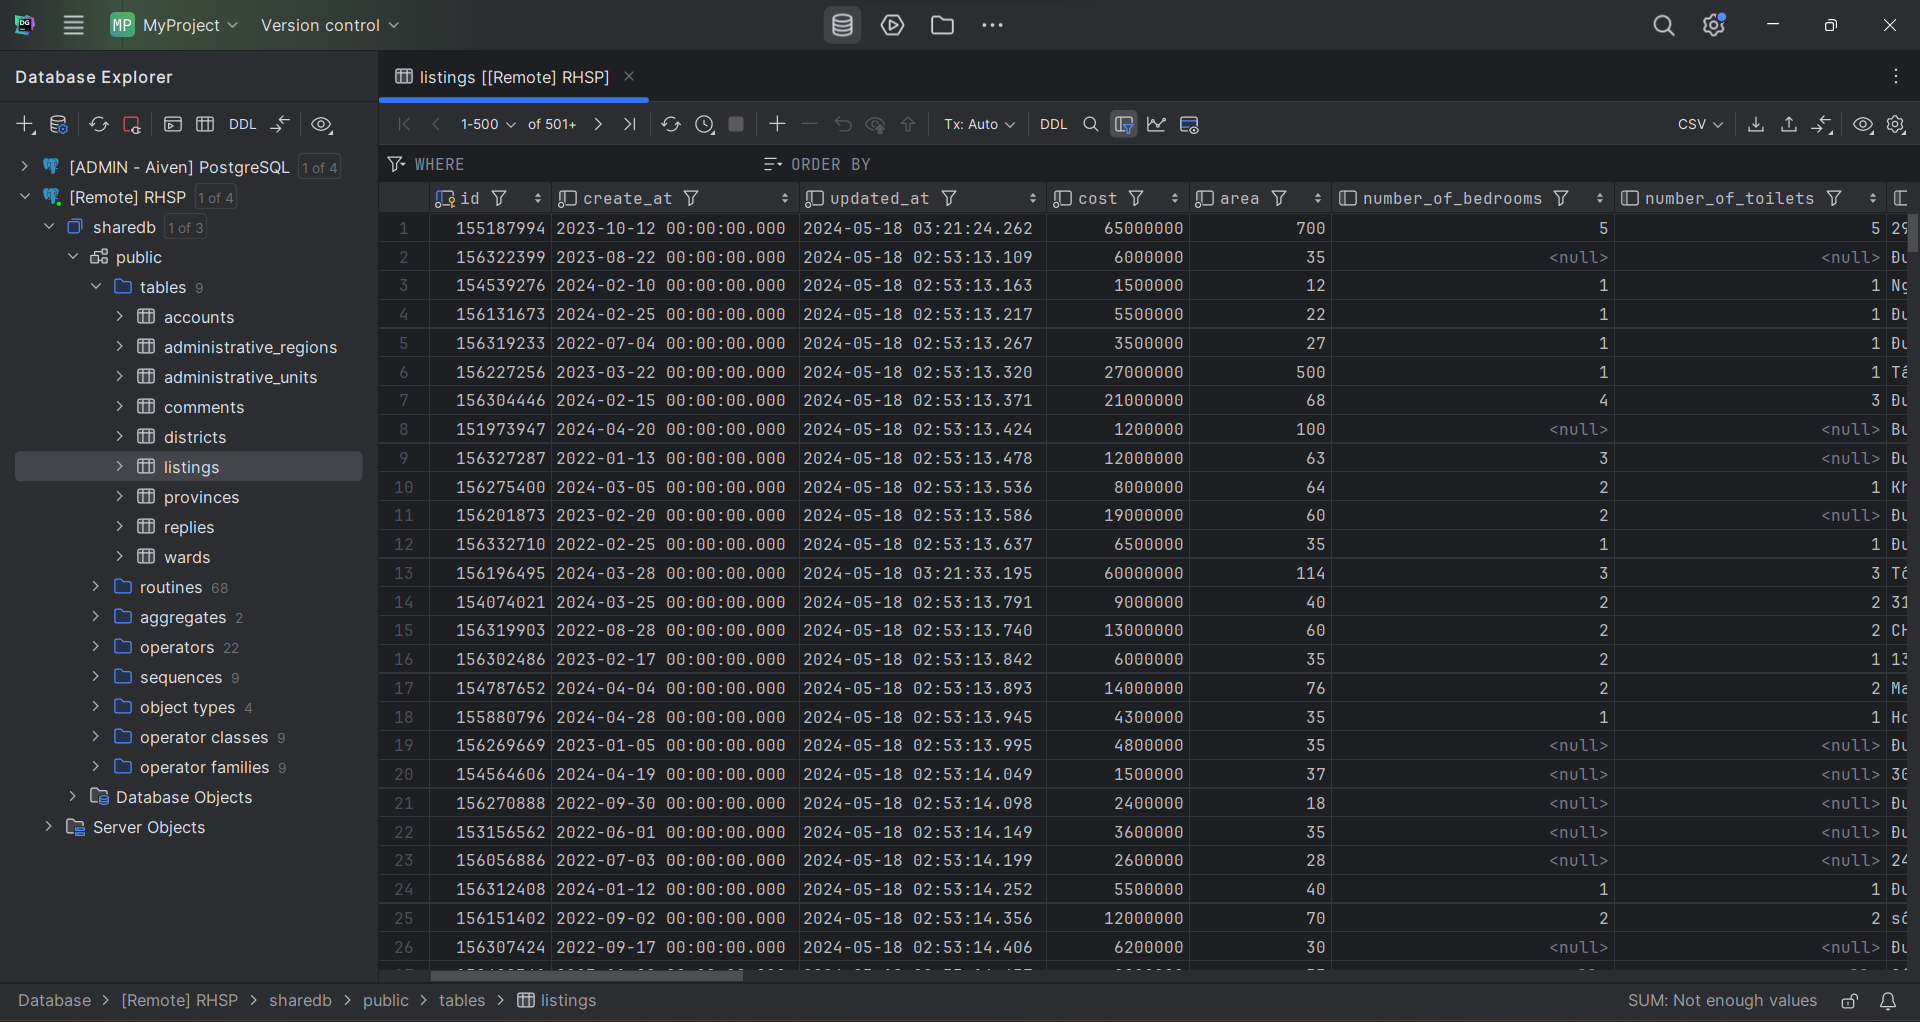
\includegraphics[width=1\textwidth]{Images/Database/DataGrip.png}
    \caption{Môi trường làm việc của DataGrip}
\end{figure}
\hspace*{1cm}
Để tạo ra thiết kế bảng cho cơ sở dữ liệu với công cụ \textit{DataGrip}, chúng ta chỉ cần nhấn chuột phải vào tên của \textit{database} hoặc \textit{schema} nằm ở cột bên trái của giao diện \textit{DataGrip}. Sau đó nhấn chọn \textit{Diagrams} và cuối cùng là nhấn chọn \textit{Show Diagram}, hoặc để đơn giản hơn, ta chỉ cần nhấn chọn chuột trái vào tên của \textit{database} hoặc \textit{schema} nằm ở cột bên trái của giao diện \textit{DataGrip}, sau đó nhấn tổ hợp phím \textit{Ctrl + Alt + Shift + U}. Sau khi thực hiện các bước trên, \textit{DataGrip} sẽ tự động tạo ra thiết kế bảng cho cơ sở dữ liệu mà ta đã chọn ở bước trên. Thiết kế bảng sẽ được hiển thị như hình ảnh bên dưới.
\begin{figure}[H]
    \centering
    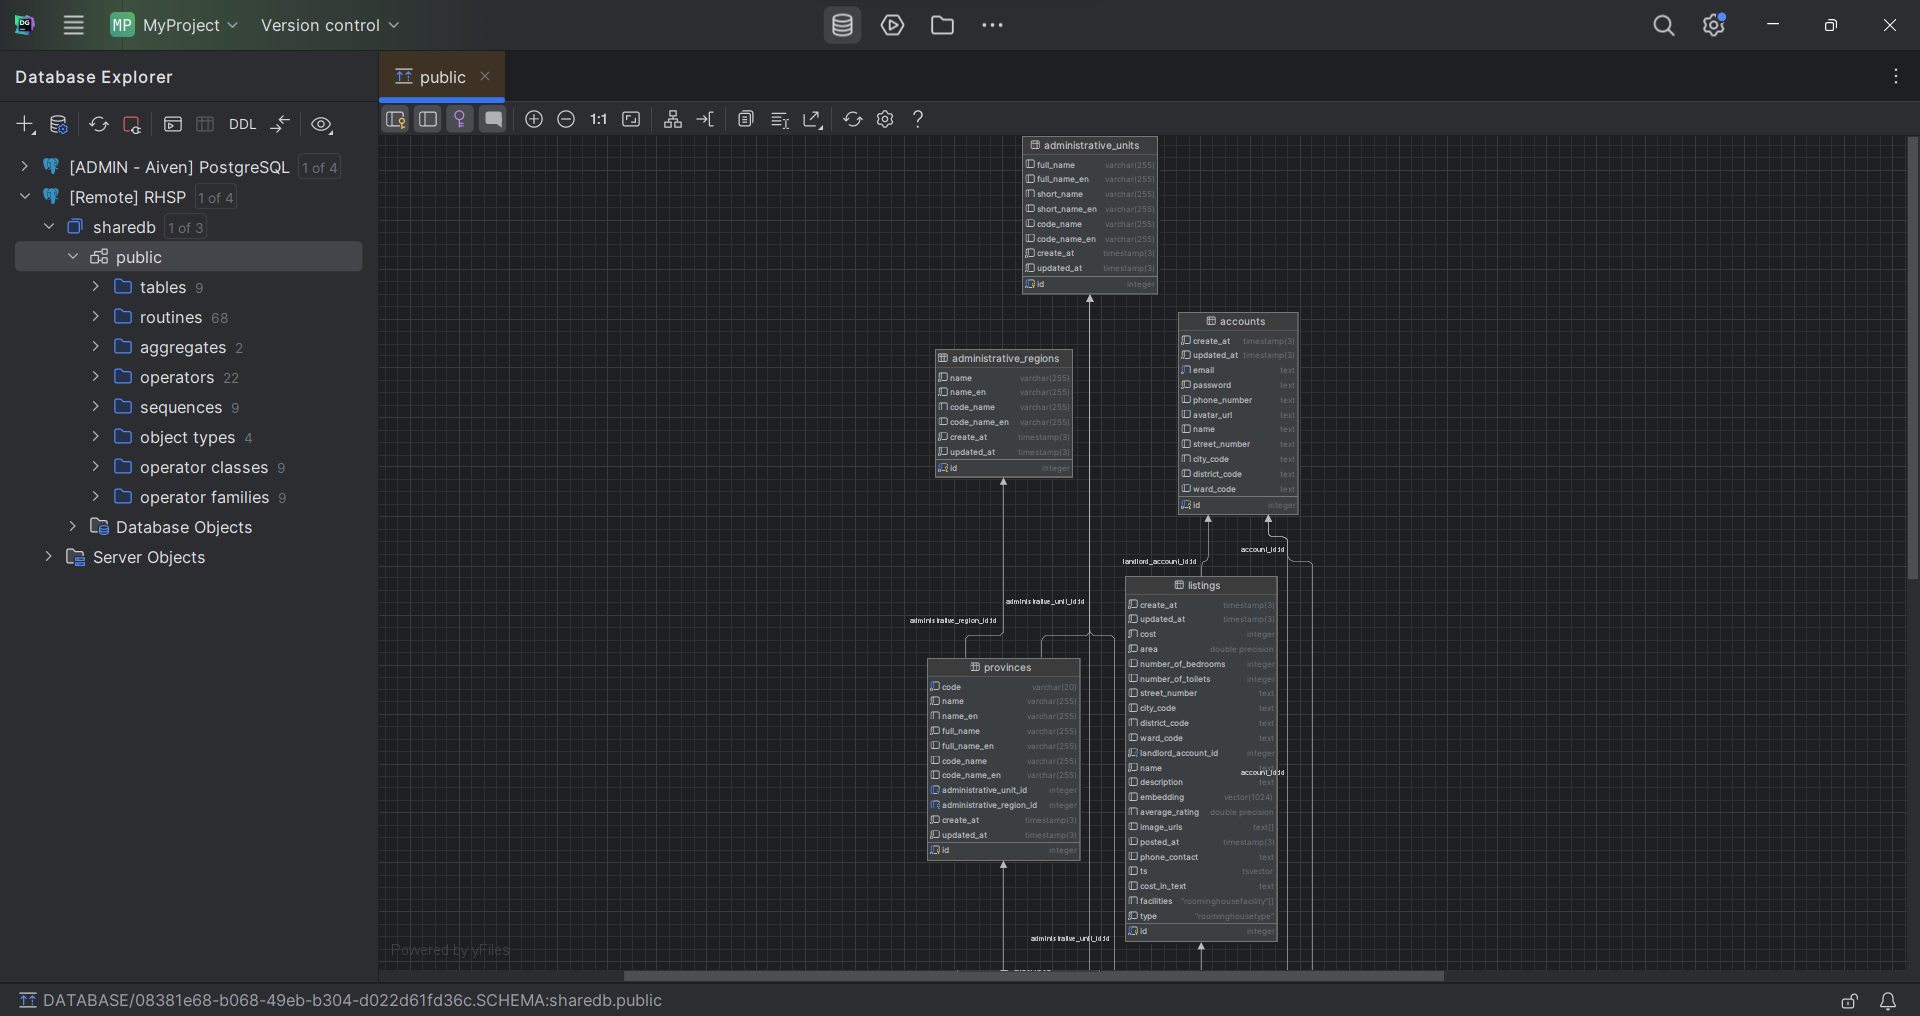
\includegraphics[width=1\textwidth]{Images/Database/ShowDiagram.png}
    \caption{Kết quả sau khi tạo thiết kế cơ sở dữ liệu trên DataGrip}
\end{figure}
\hspace*{1cm}
Do \textit{DataGrip} sinh ra thiết kế một cách tự động nên thiết kế ban đầu vẫn chưa thực sự trực quan. Ở bước này, ta cần căn chỉnh lại vị trí cho các bảng, cũng như điều chỉnh lại các đường mũi tên biểu thị cho mối quan hệ giữa các bảng với nhau để giúp cho thiết kế trở nên dễ quan sát một cách thuận tiện hơn và trực quan hơn. Sau khi đã căn chỉnh, kết quả sẽ cho ra như hình ảnh bên dưới
\begin{figure}[H]
    \centering
    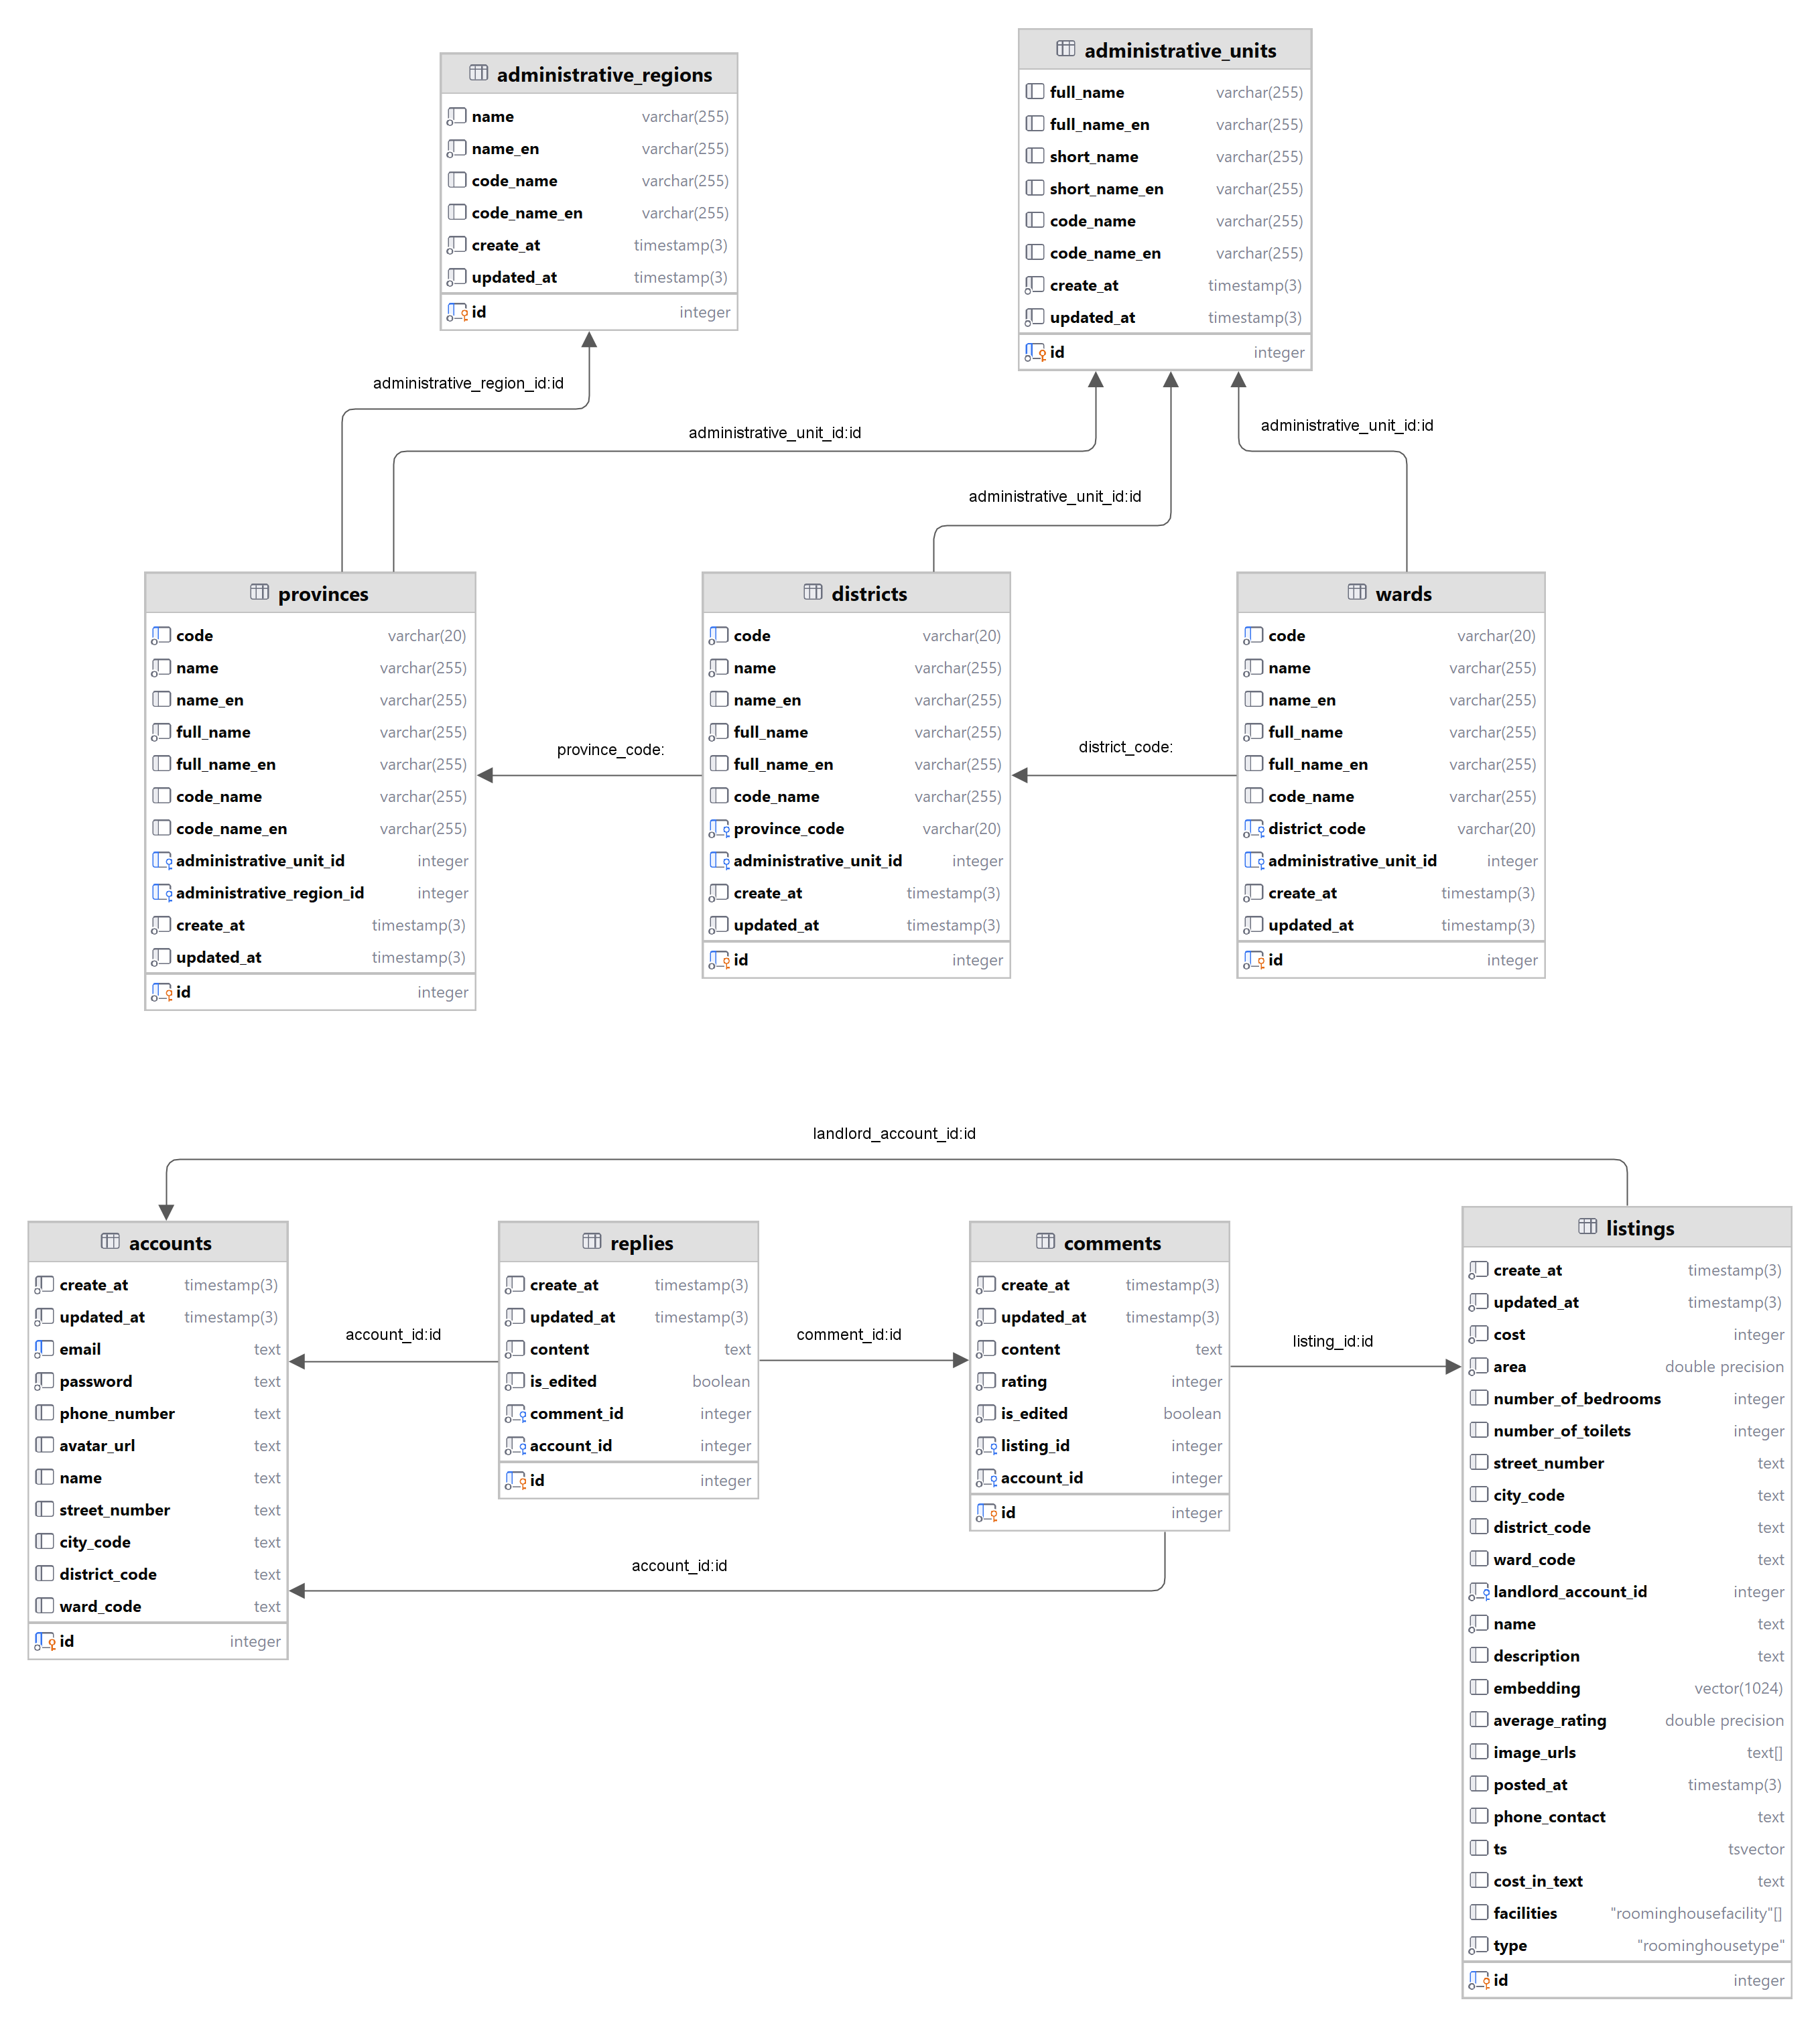
\includegraphics[width=0.98\textwidth]{Images/Database/Table.png}
    \caption{Thiết kế bảng cho cơ sở dữ liệu}
\end{figure}
\newpage
\subsection{Mô tả các bảng}
\subsubsection{Bảng administrative\_units}
\begin{center}
    \begin{longtblr}[caption={Bảng administrative\_units}]{
        colspec = { Q[m] Q[m] Q[c,m] X[m] },
        row{1} = {bg = yellow!75!black, fg = white, c},
        row{2 - 10} = {bg = yellow!10!white},
        vline{1, 5} = {2pt, yellow!75!black},
	hline{1, 2, 11} = {2pt, yellow!75!black},
        vline{2 - 4} = {dashed, yellow!75!black},
        hline{3 - 10} = {dashed, yellow!75!black},
	rows = {m},
    }
    \textbf{Thuộc tính } & \textbf{Kiểu} & \textbf{NULLABLE} & \textbf{Mô tả}
    \\
    \underline{\bf id} & integer & False & \textbf{Khóa chính}, thiết lập tự động tăng giá trị
    \\
    create\_at & timestamp(3) & False & Thời điểm khởi tạo dữ liệu, mặc định là \textit{now}
    \\
    update\_at & timestamp(3) & False & Thời điểm cuối cùng bản ghi cỏ thay đổi thuộc tính
    \\
    full\_name & varchar(100) & True & Tên đầy đủ của đơn vị hành chính
    \\
    full\_name\_en & varchar(100) & True & Tên đầy đủ của đơn vị hành chính bằng tiếng Anh
    \\
    short\_name & varchar(100) & True & Tên ngắn gọn của đơn vị hành chính
    \\
    short\_name\_en & varchar(100) & True & Tên ngắn gọn của đơn vị hành chính bằng tiếng Anh
    \\
    code\_name & varchar(100) & True & Tên chuẩn hóa của đơn vị hành chính
    \\
    code\_name\_en & varchar(100) & True & Tên chuẩn hóa của đơn vị hành chính bằng tiếng Anh
    \end{longtblr}
\end{center}
\subsubsection{Bảng administrative\_regions}
\begin{center}
    \begin{longtblr}[caption={Bảng administrative\_regions}]{
        colspec = { Q[m] Q[m] Q[c,m] X[m] },
        row{1} = {bg = yellow!75!black, fg = white, c},
        row{2 - 8} = {bg = yellow!10!white},
        vline{1, 5} = {2pt, yellow!75!black},
	hline{1, 2, 9} = {2pt, yellow!75!black},
        vline{2 - 4} = {dashed, yellow!75!black},
        hline{3 - 8} = {dashed, yellow!75!black},
	rows = {m},
    }
    \textbf{Thuộc tính } & \textbf{Kiểu} & \textbf{NULLABLE} & \textbf{Mô tả}
    \\
    \underline{\bf id} & integer & False & \textbf{Khóa chính}, thiết lập tự động tăng giá trị
    \\
    create\_at & timestamp(3) & False & Thời điểm khởi tạo dữ liệu, mặc định là \textit{now}
    \\
    update\_at & timestamp(3) & False & Thời điểm cuối cùng bản ghi cỏ thay đổi thuộc tính
    \\
    name & varchar(255) & True & Tên đầy đủ của vùng kinh tế - xã hội
    \\
    name\_en & varchar(255) & True & Tên đầy đủ của vùng kinh tế - xã hội bằng tiếng Anh
    \\
    code\_name & varchar(255) & True & Tên chuẩn hóa của  vùng kinh tế - xã hội
    \\
    code\_name\_en & varchar(255) & True & Tên chuẩn hóa của vùng kinh tế - xã hội bằng tiếng Anh
    \end{longtblr}
\end{center}
\subsubsection{Bảng province}
\begin{center}
    \begin{longtblr}[caption={Bảng province}]{
        colspec = { Q[m] Q[m] Q[c,m] X[m] },
        row{1} = {bg = yellow!75!black, fg = white, c},
        row{2 - 10} = {bg = yellow!10!white},
        vline{1, 5} = {2pt, yellow!75!black},
	hline{1, 2, 11} = {2pt, yellow!75!black},
        vline{2 - 4} = {dashed, yellow!75!black},
        hline{3 - 10} = {dashed, yellow!75!black},
	rows = {m},
    }
    \textbf{Thuộc tính } & \textbf{Kiểu} & \textbf{NULLABLE} & \textbf{Mô tả}
    \\
    \underline{\bf id} & integer & False & \textbf{Khóa chính}, thiết lập tự động tăng giá trị
    \\
    create\_at & timestamp(3) & False & Thời điểm khởi tạo dữ liệu, mặc định là \textit{now}
    \\
    update\_at & timestamp(3) & False & Thời điểm cuối cùng bản ghi cỏ thay đổi thuộc tính
    \\
    code & varchar(20) & False & Mã tỉnh / thành phố
    \\
    full\_name & varchar(255) & True & Tên đầy đủ của tỉnh / thành phố
    \\
    full\_name\_en & varchar(255) & True & Tên đầy đủ của tỉnh / thành phố bằng tiếng Anh
    \\
    code\_name & varchar(255) & True & Tên chuẩn hóa của tỉnh / thành phố
    \\
    administrative\_unit\_id & integer & False & \textit{Khóa ngoại}, tham chiếu đến \textit{id} của bảng \textbf{administrative\_units}
    \\
    administrative\_region\_id & integer & False & \textbf{Khóa ngoại}, tham chiếu đến \textit{id} của bảng \textit{administrative\_regions}
    \end{longtblr}
\end{center}
\newpage
\subsubsection{Bảng districts}
\begin{center}
    \begin{longtblr}[caption={Bảng districts}]{
        colspec = { Q[m] Q[m] Q[c,m] X[m] },
        row{1} = {bg = yellow!75!black, fg = white, c},
        row{2 - 10} = {bg = yellow!10!white},
        vline{1, 5} = {2pt, yellow!75!black},
	hline{1, 2, 11} = {2pt, yellow!75!black},
        vline{2 - 4} = {dashed, yellow!75!black},
        hline{3 - 10} = {dashed, yellow!75!black},
	rows = {m},
    }
    \textbf{Thuộc tính } & \textbf{Kiểu} & \textbf{NULLABLE} & \textbf{Mô tả}
    \\
    \underline{\bf id} & integer & False & \textbf{Khóa chính}, thiết lập tự động tăng giá trị
    \\
    create\_at & timestamp(3) & False & Thời điểm khởi tạo dữ liệu, mặc định là \textit{now}
    \\
    update\_at & timestamp(3) & False & Thời điểm cuối cùng bản ghi cỏ thay đổi thuộc tính
    \\
    code & varchar(20) & False & Mã quận / huyện và đơn vị hành chính tương đương
    \\
    full\_name & varchar(255) & True & Tên đầy đủ của quận / huyện và đơn vị hành chính tương đương
    \\
    full\_name\_en & varchar(255) & True & Tên đầy đủ của quận / huyện và đơn vị hành chính tương đương bằng tiếng Anh
    \\
    code\_name & varchar(255) & True & Tên chuẩn hóa của quận / huyện và đơn vị hành chính tương đương
    \\
    administrative\_unit\_id & integer & False & \textbf{Khóa ngoại}, tham chiếu đến trường \textit{id} của bảng \textit{administrative\_units}
    \\
    province\_code & varchar(20) & False & \textbf{Khóa ngoại}, tham chiếu đến trường \textit{code} của bảng \textit{provinces}
    \end{longtblr}
\end{center}
\subsubsection{Bảng wards}
\begin{center}
    \begin{longtblr}[caption={Bảng wards}]{
        colspec = { Q[m] Q[m] Q[c,m] X[m] },
        row{1} = {bg = yellow!75!black, fg = white, c},
        row{2 - 10} = {bg = yellow!10!white},
        vline{1, 5} = {2pt, yellow!75!black},
	hline{1, 2, 11} = {2pt, yellow!75!black},
        vline{2 - 4} = {dashed, yellow!75!black},
        hline{3 - 10} = {dashed, yellow!75!black},
	rows = {m},
    }
    \textbf{Thuộc tính } & \textbf{Kiểu} & \textbf{NULLABLE} & \textbf{Mô tả}
    \\
    \underline{\bf id} & integer & False & \textbf{Khóa chính}, thiết lập tự động tăng giá trị
    \\
    create\_at & timestamp(3) & False & Thời điểm khởi tạo dữ liệu, mặc định là \textit{now}
    \\
    update\_at & timestamp(3) & False & Thời điểm cuối cùng bản ghi cỏ thay đổi thuộc tính
    \\
    code & varchar(20) & False & Mã phường / xã và đơn vị hành chính tương đương
    \\
    full\_name & varchar(255) & True & Tên đầy đủ của phường / xã và đơn vị hành chính tương đương
    \\
    full\_name\_en & varchar(255) & True & Tên đầy đủ của phường / xã và đơn vị hành chính tương đương bằng tiếng Anh
    \\
    code\_name & varchar(255) & True & Tên chuẩn hóa của phường / xã và đơn vị hành chính tương đương
    \\
    administrative\_unit\_id & integer & False & \textit{Khóa ngoại}, tham chiếu đến trường \textbf{id} của bảng \textit{administrative\_units}
    \\
    district\_code & varchar(20) & False & \textit{Khóa ngoại}, tham chiếu đến trường \textbf{code} của bảng \textit{districts}
    \end{longtblr}
\end{center}
\subsubsection{Bảng accounts}
\begin{center}
    \begin{longtblr}[caption={Bảng accounts}]{
        colspec = { Q[m] Q[m] Q[c,m] X[m] },
        row{1} = {bg = yellow!75!black, fg = white, c},
        row{2 - 13} = {bg = yellow!10!white},
        vline{1, 5} = {2pt, yellow!75!black},
	hline{1, 2, 14} = {2pt, yellow!75!black},
        vline{2 - 4} = {dashed, yellow!75!black},
        hline{3 - 13} = {dashed, yellow!75!black},
	rows = {m},
    }
    \textbf{Thuộc tính } & \textbf{Kiểu} & \textbf{NULLABLE} & \textbf{Mô tả}
    \\
    \underline{\bf id} & int & False & \textbf{Khóa chính}, thiết lập tự động tăng giá trị
    \\
    create\_at & timestamp(3) & False & Thời điểm khởi tạo dữ liệu, mặc định là \textit{now}
    \\
    update\_at & timestamp(3) & False & Thời điểm cuối cùng bản ghi cỏ thay đổi thuộc tính
    \\
    email & text & False & Địa chỉ email của người dùng
    \\
    password & text & False & Mật khẩu của người dùng sau khi đã được băm
    \\
    name & text & True & Tên của người dùng
    \\
    avatar\_url & text & True & Đường dẫn tới file hình ảnh đại diện của người dùng
    \\
    phone\_number & text & True & Số điện thoại của người dùng
    \\
    street\_number & text & True & Số nhà và tên đường của địa chỉ người dùng
    \\
    city\_code & text & True & Mã tỉnh / thành phố của địa chỉ người dùng
    \\
    district\_code & text & True & Mã quận / huyện hoặc đơn vị hành chính tương đương của địa chỉ người dùng
    \\
    ward\_code & text & True & Mã phường / xã hoặc đơn vị hành chính tương đương của địa chỉ người dùng
    \\
    \end{longtblr}
\end{center}
\subsubsection{Bảng listings}
\begin{center}
    \begin{longtblr}[caption={Bảng listings}]{
        colspec = { Q[m] Q[m] Q[c,m] X[m] },
        row{1} = {bg = yellow!75!black, fg = white, c},
        row{2 - 22} = {bg = yellow!10!white},
        vline{1, 5} = {2pt, yellow!75!black},
	hline{1, 2, 23} = {2pt, yellow!75!black},
        vline{2 - 4} = {dashed, yellow!75!black},
        hline{3 - 22} = {dashed, yellow!75!black},
	rows = {m},
    }
    \textbf{Thuộc tính } & \textbf{Kiểu} & \textbf{NULLABLE} & \textbf{Mô tả}
    \\
    \underline{\bf id} & int & False & \textbf{Khóa chính}, thiết lập tự động tăng giá trị
    \\
    create\_at & timestamp(3) & False & Thời điểm khởi tạo dữ liệu, mặc định là \textit{now}
    \\
    update\_at & timestamp(3) & False & Thời điểm cuối cùng bản ghi cỏ thay đổi thuộc tính
    \\
    name & text & False & Tên của bài đăng tải nhà thuê
    \\
    type & rooming\_house\_type & False & Loại hình cho thuê, thuộc một
    trong các loại hình sau: \textit{Phòng trọ}, \textit{Căn hộ} hoặc \textit{Nhà đất}
    \\
    cost & integer & False & Giá tiền thuê của nhà thuê tính theo tháng
    \\
    area & double precision & False & Diện tích của nhà thuê
    \\
    number\_of\_bedrooms & integer & True & Số phòng ngủ của nhà thuê
    \\
    number\_of\_toilets & integer & True & Số nhà vệ sinh của nhà thuê
    \\
    street\_number & text & True & Số nhà và tên đường của địa chỉ nhà thuê
    \\
    city\_code & text & True & Mã tỉnh / thành phố của địa chỉ nhà thuê
    \\
    district\_code & text & True & Mã quận / huyện hoặc đơn vị hành chính tương đương của địa chỉ nhà thuê
    \\
    ward\_code & text & True & Mã phường / xã hoặc đơn vị hành chính tương đương của địa chỉ nhà thuê
    \\
    description & text & True & Mô tả ngắn về bài đăng tải nhà thuê
    \\
    image\_url & text & True & Đường dẫn tới các file hình ảnh của bài đẳng tải nhà thuê
    \\
    phone\_contact & text & True & Số điện thoại liên hệ của bài đăng tải nhà thuê
    \\
    facilities & rooming\_house\_facility & True & Các tiện ích của nhà thuê, các tiện ích đó bao gồm: \textit{Tivi}, \textit{Camera giám sát}, \textit{Cảm biến}, \textit{Tủ lạnh}, \textit{Máy giặt}, \textit{Điều hòa}
    \\
    average\_rating & text & True & Điểm đánh giá trung bình dựa trên các bình luận của bài đăng tải nhà thuê
    \\
    cost\_in\_text & text & True & Giá thuê theo tháng được phiên âm thành tiếng Việt, được sử dụng trong mô hình tìm kiếm Hybrid
    \\
    ts & tsvector & True & Lưu trữ \textit{indexes} của các từ trong bài đăng, được sử dụng trong \textit{full-text search}
    \\
    embedding & vector(1024) & True & Vector có 1024 do mô hình \textit{vector embeeding} sinh ra để biểu thị cho ngữ nghĩa của bài đăng tải nhà trọ, được sử dụng trong \textit{semantic search}
    \end{longtblr}
\end{center}
\subsubsection{Bảng comments}
\begin{center}
    \begin{longtblr}[caption={Bảng comments}]{
        colspec = { Q[m] Q[m] Q[c,m] X[m] },
        row{1} = {bg = yellow!75!black, fg = white, c},
        row{2 - 9} = {bg = yellow!10!white},
        vline{1, 5} = {2pt, yellow!75!black},
	hline{1, 2, 10} = {2pt, yellow!75!black},
        vline{2 - 4} = {dashed, yellow!75!black},
        hline{3 - 9} = {dashed, yellow!75!black},
	rows = {m},
    }
    \textbf{Thuộc tính } & \textbf{Kiểu} & \textbf{NULLABLE} & \textbf{Mô tả}
    \\
    \underline{\bf id} & int & False & \textbf{Khóa chính}, thiết lập tự động tăng giá trị
    \\
    create\_at & timestamp(3) & False & Thời điểm khởi tạo dữ liệu, mặc định là \textit{now}
    \\
    update\_at & timestamp(3) & False & Thời điểm cuối cùng bản ghi cỏ thay đổi thuộc tính
    \\
    content & text & False & Nội dung bình luận của người dùng
    \\
    rating & integer & False & Số điểm đánh giá của người dùng đối với nhà thuê
    \\
    is\_edited & boolean & False & Biểu thị cho thấy bình luận đã được chỉnh sửa hay chưa, giá trị mặc định là \textit{false}
    \\
    listing\_id & integer & False & \textbf{Khóa ngoại}, tham chiếu đến trường \textit{id} của bảng \textit{listings}
    \\
    account\_id & integer & False & \textbf{Khóa ngoại}, tham chiếu đến trường \textit{id} của bảng \textit{accounts}
    \end{longtblr}
\end{center}
\subsubsection{Bảng replies}
\begin{center}
    \begin{longtblr}[caption={Bảng replies}]{
        colspec = { Q[m] Q[m] Q[c,m] X[m] },
        row{1} = {bg = yellow!75!black, fg = white, c},
        row{2 - 8} = {bg = yellow!10!white},
        vline{1, 5} = {2pt, yellow!75!black},
	hline{1, 2, 9} = {2pt, yellow!75!black},
        vline{2 - 4} = {dashed, yellow!75!black},
        hline{3 - 8} = {dashed, yellow!75!black},
	rows = {m},
    }
    \textbf{Thuộc tính } & \textbf{Kiểu} & \textbf{NULLABLE} & \textbf{Mô tả}
    \\
    \underline{\bf id} & int & False & \textbf{Khóa chính}, thiết lập tự động tăng giá trị
    \\
    create\_at & timestamp(3) & False & Thời điểm khởi tạo dữ liệu, mặc định là \textit{now}
    \\
    update\_at & timestamp(3) & False & Thời điểm cuối cùng bản ghi cỏ thay đổi thuộc tính
    \\
    content & text & False & Nội dung trả lời phản hồi của bình luận của người dùng
    \\
    is\_edited & boolean & False & Biểu thị cho thấy phản hồi bình luận đã được chỉnh sửa hay chưa, giá trị mặc định là \textit{false}
    \\
    comment\_id & integer & False & \textbf{Khóa ngoại}, tham chiếu đến trường \textit{id} của bảng \textit{comments}
    \\
    account\_id & integer & False & \textbf{Khóa ngoại}, tham chiếu đến trường \textit{id} của bảng \textit{accounts}
    \end{longtblr}
\end{center}